\documentclass[onesided]{article}\usepackage[]{graphicx}\usepackage[]{color}
% maxwidth is the original width if it is less than linewidth
% otherwise use linewidth (to make sure the graphics do not exceed the margin)
\makeatletter
\def\maxwidth{ %
  \ifdim\Gin@nat@width>\linewidth
    \linewidth
  \else
    \Gin@nat@width
  \fi
}
\makeatother

\definecolor{fgcolor}{rgb}{0.345, 0.345, 0.345}
\newcommand{\hlnum}[1]{\textcolor[rgb]{0.686,0.059,0.569}{#1}}%
\newcommand{\hlstr}[1]{\textcolor[rgb]{0.192,0.494,0.8}{#1}}%
\newcommand{\hlcom}[1]{\textcolor[rgb]{0.678,0.584,0.686}{\textit{#1}}}%
\newcommand{\hlopt}[1]{\textcolor[rgb]{0,0,0}{#1}}%
\newcommand{\hlstd}[1]{\textcolor[rgb]{0.345,0.345,0.345}{#1}}%
\newcommand{\hlkwa}[1]{\textcolor[rgb]{0.161,0.373,0.58}{\textbf{#1}}}%
\newcommand{\hlkwb}[1]{\textcolor[rgb]{0.69,0.353,0.396}{#1}}%
\newcommand{\hlkwc}[1]{\textcolor[rgb]{0.333,0.667,0.333}{#1}}%
\newcommand{\hlkwd}[1]{\textcolor[rgb]{0.737,0.353,0.396}{\textbf{#1}}}%
\let\hlipl\hlkwb

\usepackage{framed}
\makeatletter
\newenvironment{kframe}{%
 \def\at@end@of@kframe{}%
 \ifinner\ifhmode%
  \def\at@end@of@kframe{\end{minipage}}%
  \begin{minipage}{\columnwidth}%
 \fi\fi%
 \def\FrameCommand##1{\hskip\@totalleftmargin \hskip-\fboxsep
 \colorbox{shadecolor}{##1}\hskip-\fboxsep
     % There is no \\@totalrightmargin, so:
     \hskip-\linewidth \hskip-\@totalleftmargin \hskip\columnwidth}%
 \MakeFramed {\advance\hsize-\width
   \@totalleftmargin\z@ \linewidth\hsize
   \@setminipage}}%
 {\par\unskip\endMakeFramed%
 \at@end@of@kframe}
\makeatother

\definecolor{shadecolor}{rgb}{.97, .97, .97}
\definecolor{messagecolor}{rgb}{0, 0, 0}
\definecolor{warningcolor}{rgb}{1, 0, 1}
\definecolor{errorcolor}{rgb}{1, 0, 0}
\newenvironment{knitrout}{}{} % an empty environment to be redefined in TeX

\usepackage{alltt}
\usepackage[T1]{fontenc}
\linespread{1.5} % Line spacing - Palatino needs more space between lines
\usepackage{microtype} % Slightly tweak font spacing for aesthetics

\usepackage[hmarginratio=1:1,columnsep=20pt]{geometry} % Document margins
%\usepackage{multicol} % Used for the two-column layout of the document
\usepackage[hang, small,labelfont=bf,up,textfont=it,up]{caption} % Custom captions under/above floats in tables or figures
\usepackage{booktabs} % Horizontal rules in tables
\usepackage{float} % Required for tables and figures in the multi-column environment - they need to be placed in specific locations with the [H] (e.g. \begin{table}[H])

\usepackage{lettrine} % The lettrine is the first enlarged letter at the beginning of the text
\usepackage{paralist} % Used for the compactitem environment which makes bullet points with less space between them

% to ignore texts: good for thank messages and paper submissions.
      % \fbox{\phantom{This text will be invisible too, but a box will be printed arround it.}}

\usepackage{abstract} % Allows abstract customization
\renewcommand{\abstractnamefont}{\normalfont\bfseries} % Set the "Abstract" text to bold
%\renewcommand{\abstracttextfont}{\normalfont\small\itshape} % Set the abstract itself to small italic text

\usepackage[]{titlesec} % Allows customization of titles
\renewcommand\thesection{\Roman{section}} % Roman numerals for the sections
\renewcommand\thesubsection{\Roman{subsection}} % Roman numerals for subsections
\titleformat{\section}[block]{\large\scshape\centering}{\thesection.}{1em}{} % Change the look of the section titles
\titleformat{\subsection}[block]{\large}{\thesubsection.}{1em}{} % Change the look of the section titles

\usepackage{fancybox, fancyvrb, calc}
\usepackage[svgnames]{xcolor}
\usepackage{physics}
\usepackage{epigraph}
\usepackage{longtable}
\usepackage{pdflscape}
\usepackage{graphics}
\usepackage{pbox} % \pbox{20cm}{This is the first \\ cell}
\usepackage{amsfonts}
\usepackage{amsmath}
\usepackage{amssymb}
\usepackage{rotating}
\usepackage{paracol}
\usepackage{textcomp}
\usepackage[export]{adjustbox}
\usepackage{afterpage}
\usepackage{filecontents}
\usepackage{color}
\usepackage{latexsym}
\usepackage{lscape}       %\begin{landscape} and \end{landscape}
\usepackage{wasysym}
\usepackage{dashrule}
\usepackage{marvosym} % face package
\usepackage{framed}
\usepackage{tree-dvips}
\usepackage{pgffor}
\usepackage[]{authblk}
\usepackage{setspace}
\usepackage{array}
\usepackage[latin1]{inputenc}
\usepackage{hyperref}     %desactivar para link rojos
\usepackage{graphicx}
\usepackage{dcolumn} % for R tables
\usepackage{multirow} % For multirow in tables
\usepackage{pifont}
\usepackage{listings}
\usepackage{bm}




% hypothesis / theorem package begin
\usepackage{amsthm}
\usepackage{thmtools}
\declaretheoremstyle[
spaceabove=6pt, spacebelow=6pt,
headfont=\normalfont\bfseries,
notefont=\mdseries, notebraces={(}{)},
bodyfont=\normalfont,
postheadspace=0.6em,
headpunct=:
]{mystyle}
\declaretheorem[style=mystyle, name=Hypothesis, preheadhook={\renewcommand{\thehyp}{H\textsubscript{\arabic{hyp}}}}]{hyp}

\usepackage{cleveref}
\crefname{hyp}{hypothesis}{hypotheses}
\Crefname{hyp}{Hypothesis}{Hypotheses}
% hypothesis / theorem package end


%----------------------------------------------------------------------------------------
% Other ADDS-ON
%----------------------------------------------------------------------------------------

% independence symbol \independent
\newcommand\independent{\protect\mathpalette{\protect\independenT}{\perp}}
\def\independenT#1#2{\mathrel{\rlap{$#1#2$}\mkern2mu{#1#2}}}







\hypersetup{
    bookmarks=true,         % show bookmarks bar?
    unicode=false,          % non-Latin characters in Acrobat's bookmarks
    pdftoolbar=true,        % show Acrobat's toolbar?
    pdfmenubar=true,        % show Acrobat's menu?
    pdffitwindow=true,     % window fit to page when opened
    pdfstartview={FitH},    % fits the width of the page to the window
    pdftitle={My title},    % title
    pdfauthor={Author},     % author
    pdfsubject={Subject},   % subject of the document
    pdfcreator={Creator},   % creator of the document
    pdfproducer={Producer}, % producer of the document
    pdfkeywords={keyword1} {key2} {key3}, % list of keywords
    pdfnewwindow=true,      % links in new window
    colorlinks=true,       % false: boxed links; true: colored links
    linkcolor=ForestGreen,          % color of internal links (change box color with linkbordercolor)
    citecolor=ForestGreen,        % color of links to bibliography
    filecolor=ForestGreen,      % color of file links
    urlcolor=ForestGreen           % color of external links
}

%\usepackage[nodayofweek,level]{datetime} % to have date within text

\newcommand{\LETT}[3][]{\lettrine[lines=4,loversize=.2,#1]{\smash{#2}}{#3}} % letrine customization



% comments on margin
  % Select what to do with todonotes: 
  % \usepackage[disable]{todonotes} % notes not showed
  \usepackage[draft]{todonotes}   % notes showed
  % usage: \todo{This is a note at margin}

\usepackage{cooltooltips}

%%% bib begin
\usepackage[american]{babel}
\usepackage{csquotes}
\usepackage[backend=biber,style=authoryear,dashed=false,doi=false,isbn=false,url=false,arxiv=false]{biblatex}
%\DeclareLanguageMapping{american}{american-apa}
\addbibresource{/Users/hectorbahamonde/Bibliografia_PoliSci/library.bib} 
\addbibresource{/Users/hectorbahamonde/Bibliografia_PoliSci/Bahamonde_BibTex2013.bib} 

% USAGES
%% use \textcite to cite normal
%% \parencite to cite in parentheses
%% \footcite to cite in footnote
%% the default can be modified in autocite=FOO, footnote, for ex. 
%%% bib end

\usepackage{fancyhdr} % Headers and footers
\pagestyle{fancy} % All pages have headers and footers
\fancyhead{} % Blank out the default header
\fancyfoot{} % Blank out the default footer
\fancyhead[C]{MLE y Causal Inference: Matching, Covariate Balance, y el Propensity Score} % Custom header text
\fancyfoot[RO,LE]{\thepage} % Custom footer text
\IfFileExists{upquote.sty}{\usepackage{upquote}}{}
\begin{document}
% DOCUMENT ID
%----------------------------------------------------------------------------------------
%	CONTENT
%----------------------------------------------------------------------------------------

%\graphicspath{
%{/Users/hectorbahamonde/RU/Term5/Experiments_Redlawsk/Experiment/Data/}
%}



%%%%%%%%%%%%%%%%%%%%%%%%%%%%%%%%%%%%%%%%%%%%%%
% begin knitr stuff


%%%%%%%%%%%%%%%%%%%%%%%%%%%%%%%%%%%%%%%%%%%%%%





\hspace{-5mm}{\bf Profesor}: H\'ector Bahamonde, PhD.\\
\texttt{e:}\href{mailto:hector.bahamonde@uoh.cl}{\texttt{hector.bahamonde@uoh.cl}}\\
\texttt{w:}\href{http://www.hectorbahamonde.com}{\texttt{www.hectorbahamonde.com}}\\
{\bf Curso}: MLE.\\
\hspace{-5mm}{\bf TA}: Gonzalo Barr\'ia.

\section{MLE y Causal Inference: Matching, Covariate Balance, y el Propensity Score}

\paragraph{Motivaci\'on} De acuerdo a \textcite[33]{Morgan:2007ty}, el \emph{treatment effect} (TE) ``naive'' $\delta_{i}$ para el sujeto $i$ es,

\begin{equation}\label{eqMETH:1}
\delta_{i} = y^{\texttt{T}}_{i} - y^{\texttt{C}}_{i}
\end{equation}

\paragraph{}donde $y$ es la variable dependiente bajo un r\'egimen de tratamiento (\texttt{T}) o control (\texttt{C}). Como ya sabemos, este TE es ``naive'' en el sentido de que es una cantidad de inter\'es no observada: es imposible observar los dos estados para el mismo sujeto $i$. O ves uno o ves el otro. Esto es lo que de manera muy conocida \textcite[947]{Holland1986a} ha llamado el \emph{fundamental problem of causal inference}.

\paragraph{}Es por esto que nosotros trabajamos con el \emph{average treatment effect} (ATE).

\begin{equation}\label{eqMETH:2}
\text{ATE} = \frac{1}{n}\sum^{n}_{i=1} E[Y_{i}^{\texttt{T}}-Y_{i}^{\texttt{C}} \;|\; X_{i} ]
\end{equation}


Como ves, el efecto causal ``{\bf average}'' es la resta del grupo que fue tratado  (\texttt{T})  menos el grupo que no fue tratado (\texttt{C}) \parencite[204]{Ho2006}.

La l\'ogica experimental indica que en vez de controlar por \emph{covariados} (como se hace en una regresi\'on lineal tipo OLS), controlas por nada \parencite[6]{Guo:2009il}. Lo que termina ``controlando'' es la aleatorizaci\'on del r\'egimen experimental (\texttt{T} o \texttt{C}). {\color{red}Por qu\'e?} Lo que logra la randomizaci\'on, de manera m\'as formal, es lo siguiente:

\begin{equation}\label{eqMETH:5b}
i \independent \text{\texttt{C}}, \text{\texttt{T}}
\end{equation}

En palabras, la asignaci\'on de la unidad $i$ a uno de los dos r\'egimenes es \emph{independiente} (``$\independent$'') de las c\'aracteristicas de la unidad $i$. {\color{red}Por qu\'e esto es importante?}.

Aunque es claro que todos quisi\'eramos realizar experimentos para poder calcular el ATE en \autoref{eqMETH:2}, esto s\'olo es posible en contextos experimentales. En el resto de las veces (observacional), esto no ser\'a posible. Muchas veces los experimentos no est\'an disponibles debido a la imposibilidad de hacer uno (costo, criterios \'eticos, etc.). {\bf C\'omo podemos ``simular'' un experimento cuando no podemos conseguir uno?} Una t\'ecnica posible es el ``{\bf matching}''.

\paragraph{``Covariate Balance''} Lo que la randomizaci\'on experimental logra es \emph{covariate balance}, es decir, que \emph{{\bf TODAS}} las caracter\'isticas \emph{pre-treatment} sean balanceadas en los dos reg\'imenes experimentales. Es decir, todo lo que observamos de $i$ (y lo que \emph{no} observamos tambi\'en) estar\'a distribuido de igual manera (i.e. ``balanceado'') en ambos reg\'imenes. El \emph{covariate balance} es fundamental porque hace que las caracter\'isticas de todos los $i$ (genero, ingresos, ideolog\'ia, etc.) est\'en distribuidas de igual maneras. Lo importante es que cuando eso ocurre, las diferencias (entre genero, por ejemplo) se cancelar\'an entre ellas. Lo mismo ocurre con todo el resto de carecter\'isticas (observables y no-observables). {\color{red}Qu\'e ventajas trae esto en relaci\'on a la regresi\'on?}

Lo que hace el {\bf matching} es encontrar \emph{pares similares} (o ``matches'') entre el grupo \texttt{C} y el grupo \texttt{T}. La idea es lograr ({\bf usando datos observacionales}) el \emph{covariate balance} que logra un experimento (sin tener uno). 

\paragraph{Propensity Score Matching} Las t\'ecnicas de \emph{matching} trabajan con {\bf distancias} que indican cu\'an iguales o diferentes son las unidades $i$.\footnote{Hay varias clases de distancias. En esta clase s\'olo veremos el \emph{propensisty score}.} Es sobre esas distancias que determinamos si una unidad $i_{\texttt{T}}$ encuentra su ``\emph{match}'' $i_{\texttt{C}}$. La distancia m\'as usada es el ``\emph{propensity score}'' (PS). {\bf El PS es la probabilidad de $i$ de ser asignado al r\'egimen \texttt{T}}. Si conocemos estas probabilidades, podemos tratar de imitar un experimento (pero usando datos observacionales), espec\'ificamente, en lo que respecta al \emph{covariate balance}. Si conocemos la probabilidad de ser asignado al tratamiento (que es la definici\'on del PS), podemos balancear nuestros datos y {\bf botar} todas las observaciones que no encuentren su \emph{match} (en funci\'on de la probabilidad del PS). Al botar observaciones que no tengan pares similares en cuanto al PS estaremos {\bf balanceando nuestros datos}. Y es que de esta manera imitamos un experimento cuando no podemos realizar uno.


M\'as formalmente, lo que nosotros queremos lograr es que la variable dependiente $y$ sea ``ortogonal'' (o independiente, i.e. $\independent$) del mecanismo de asignaci\'on al tratamiento $\tau$---un experimento logra eso de manera natural, no as\'i un dise\~no observacional donde puede que exista una correlaci\'on $\text{Corr}(y,\tau)>0$. El PS ayuda a que, cuando es condicionado en el \emph{propensity score} (o ``\emph{balancing score}'') $b(X)$ $y$ sea ortogonal a $\tau$, de manera tal que,

\begin{equation}\label{eqMETH:7}
y_{i} \independent \tau_{i} | x_{i} \equiv y_{i} \independent \tau_{i} | b(X)_{i}
\end{equation}

Estad\'istiamente, lo que ocurre al balancear $y_{i}$ en cuanto al PS $b(X)_{i}$ es que ambas distribuciones se hacen indistinguibles. {\color{red}Por qu\'e?} Y eso es justamente lo que buscamos: que ambos grupos \texttt{T} y \texttt{C} sean iguales, excepto en $\tau_{i}$. Piensa en un experimento: ambos grupos (\texttt{T}, \texttt{C}) son iguales (por el efecto de la randomizaci\'on), {\bf \emph{excepto}} en que un $i_{\texttt{T}}$ es tratado y el otro $i_{\texttt{C}}$ no es tratado. 

Claramente, todo esto supone que nosotros conocemos (o al menos, podemos construir) el PS. Para hacerlo, debemos estimar una regresi\'on log\'istica. La variable dependiente es el vector $\tau_{0,1}$ y las variables independientes est\'an compuestas por una matriz $x$ que contenga caracter\'isticas \emph{pre-treatment}. Formalmente, necesitamos estimar,

\begin{equation}\label{logit.structural}
\tau = \boldsymbol{x_{i}}\boldsymbol{\beta} + \epsilon_{i}
\end{equation}

donde $\boldsymbol{x_{i}}$ es la matriz $x$ que contiene caracter\'isticas \emph{pre-treatment}. Nota que $\tau \sim \text{Logistic}(\mu, \frac{\sigma^{2}\pi^{2}}{3})$, y donde $\sigma^{2}$ es proporcional a la desviaci\'on est\'andard.

\paragraph{``\emph{Matching} as a Preprocessing Tool''} \textcite{Ho2006} explica que {\bf \emph{matching} se debe ocupar como una herramienta para pre-procesar los datos}. Recuerda que \emph{matching}, lo que esencialmente hace, es botar observaciones. \emph{Matching} no es una herramienta de inferencia estad\'istica propiamente tal. En consecuencia, los autores recomiendan hacer \emph{matching} {\bf antes} de estimar cualquier modelo param\'etrico. La idea es primero obtener datos quasi-experimentales (v\'ia \emph{matching}) y despu\'es estimar modelos OLS o GLM (u otros). 

\begin{itemize}
\item {\bf Ventajas}:
		\begin{enumerate}
			\item Una base de datos pre-procesada es menos dependiente del modelo. {\color{red}Por qu\'e es esto importante?}
			\item Nos acercamos a un dise\~no experimental.
		\end{enumerate}
\item {\bf Desventajas}:
		\begin{enumerate}
			\item El PS es altamente dependiente de los \emph{pre-treatment covariates} $x$. 
			\item El PS ``se vende'' como no-parametrico, i.e. libre de supuestos distribucionales e inferenciales. {\color{red}Es?}
			\item Matching selecciona en observables. La experimentaci\'on en observables y no-observables.
			\item Existen muchas distancias: poca claridad de un metodo unico de \emph{matching}. Cacofon\'ia.
		\end{enumerate}
\end{itemize}

\subsection{Estimaci\'on}

Estimemos modelos sin \emph{matching} (``raw'') y con \emph{matching}. Simulemos unos datos.


\begin{knitrout}
\definecolor{shadecolor}{rgb}{0.969, 0.969, 0.969}\color{fgcolor}\begin{kframe}
\begin{alltt}
\hlkwd{set.seed}\hlstd{(}\hlnum{2020}\hlstd{)} \hlcom{# seed}
\hlcom{#}
\hlstd{e} \hlkwb{=} \hlkwd{rnorm}\hlstd{(}\hlnum{1100}\hlstd{,} \hlnum{0}\hlstd{)} \hlcom{# residuo }
\hlstd{x1} \hlkwb{=} \hlkwd{rnorm}\hlstd{(}\hlnum{1100}\hlstd{,} \hlopt{-}\hlnum{10}\hlstd{)} \hlcom{# x1}
\hlstd{x2} \hlkwb{=} \hlkwd{rnorm}\hlstd{(}\hlnum{1100}\hlstd{,} \hlnum{20}\hlstd{)} \hlcom{# x2}
\hlcom{# mecanismo de asignacion a tratamiento sesgado: depende de x1 y una constante.}
\hlstd{t} \hlkwb{<-} \hlkwd{as.numeric}\hlstd{(}\hlnum{1} \hlopt{+} \hlnum{0.02}\hlopt{*}\hlstd{x1)}
\hlstd{pr} \hlkwb{=} \hlkwd{as.numeric}\hlstd{(}\hlnum{1}\hlopt{/}\hlstd{(}\hlnum{1}\hlopt{+}\hlkwd{exp}\hlstd{(}\hlopt{-}\hlstd{t)))} \hlcom{# poner t en una funcion logit invertida}
\hlstd{z} \hlkwb{=} \hlkwd{rbinom}\hlstd{(}\hlnum{1100}\hlstd{,}\hlnum{1}\hlstd{,pr)} \hlcom{# crear z como funcion binomial basado en el vector de prob's}
\hlcom{#}
\hlstd{y} \hlkwb{<-} \hlkwd{as.numeric}\hlstd{(}\hlnum{1}\hlopt{*}\hlstd{z} \hlopt{+} \hlnum{1}\hlopt{*}\hlstd{x1} \hlopt{+} \hlnum{2}\hlopt{*}\hlstd{x2} \hlopt{+} \hlstd{e)} \hlcom{# y es combinacion lineal de factores}
\hlcom{#}
\hlstd{dat} \hlkwb{=} \hlkwd{as.data.frame}\hlstd{(}\hlkwd{cbind}\hlstd{(y, x1, x2,z))} \hlcom{# crear base de datos}
\end{alltt}
\end{kframe}
\end{knitrout}

Veamos la distribuci\'on de $z$. 

\begin{knitrout}
\definecolor{shadecolor}{rgb}{0.969, 0.969, 0.969}\color{fgcolor}\begin{kframe}
\begin{alltt}
\hlkwd{library}\hlstd{(lattice)}
\hlkwd{histogram}\hlstd{(z)}
\end{alltt}
\end{kframe}

{\centering 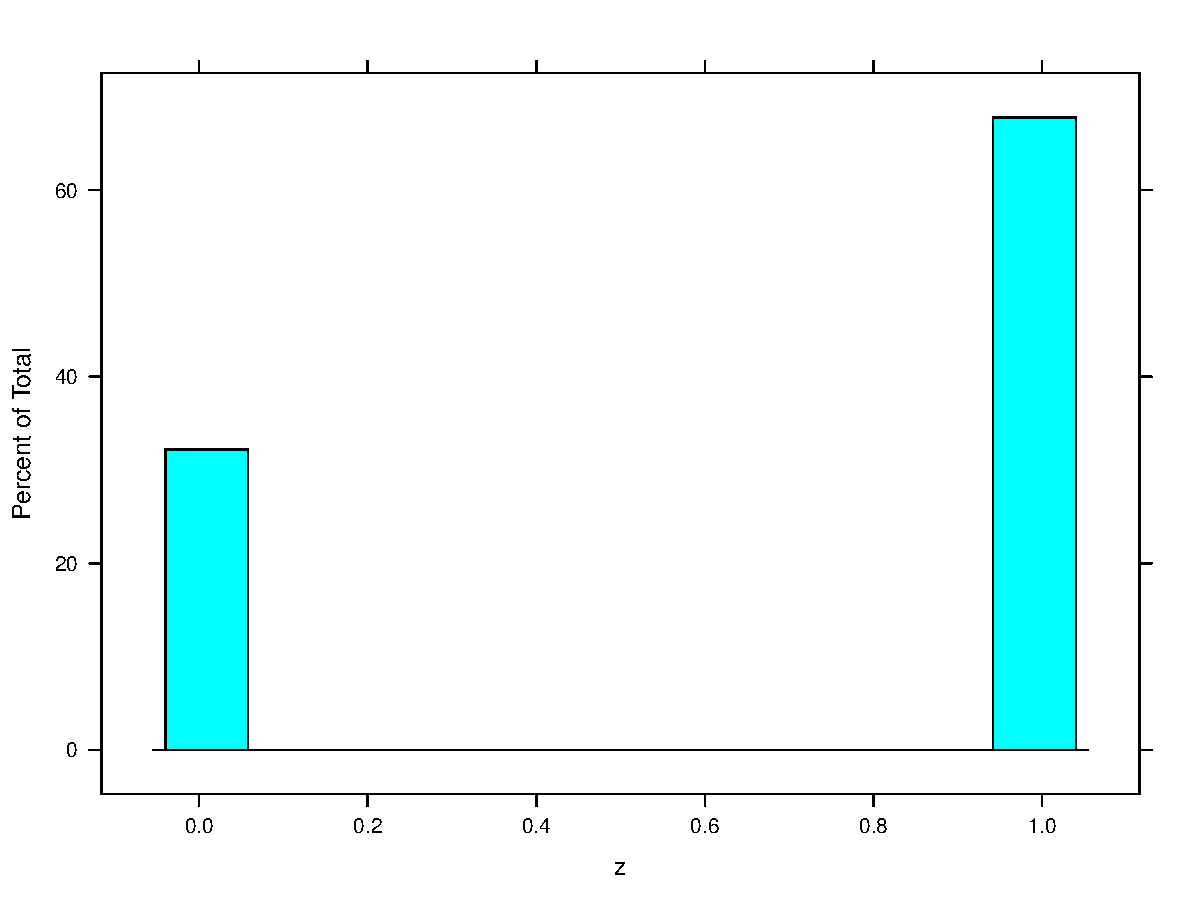
\includegraphics[width=\maxwidth]{figure/sim:2-1} 

}



\end{knitrout}

Veamos el \emph{imbalance} de los covariados.

\begin{knitrout}
\definecolor{shadecolor}{rgb}{0.969, 0.969, 0.969}\color{fgcolor}\begin{kframe}
\begin{alltt}
\hlkwd{library}\hlstd{(lattice)}
\hlkwd{densityplot}\hlstd{(x1,} \hlkwc{groups} \hlstd{= z,} \hlkwc{data} \hlstd{= dat)}
\end{alltt}
\end{kframe}

{\centering 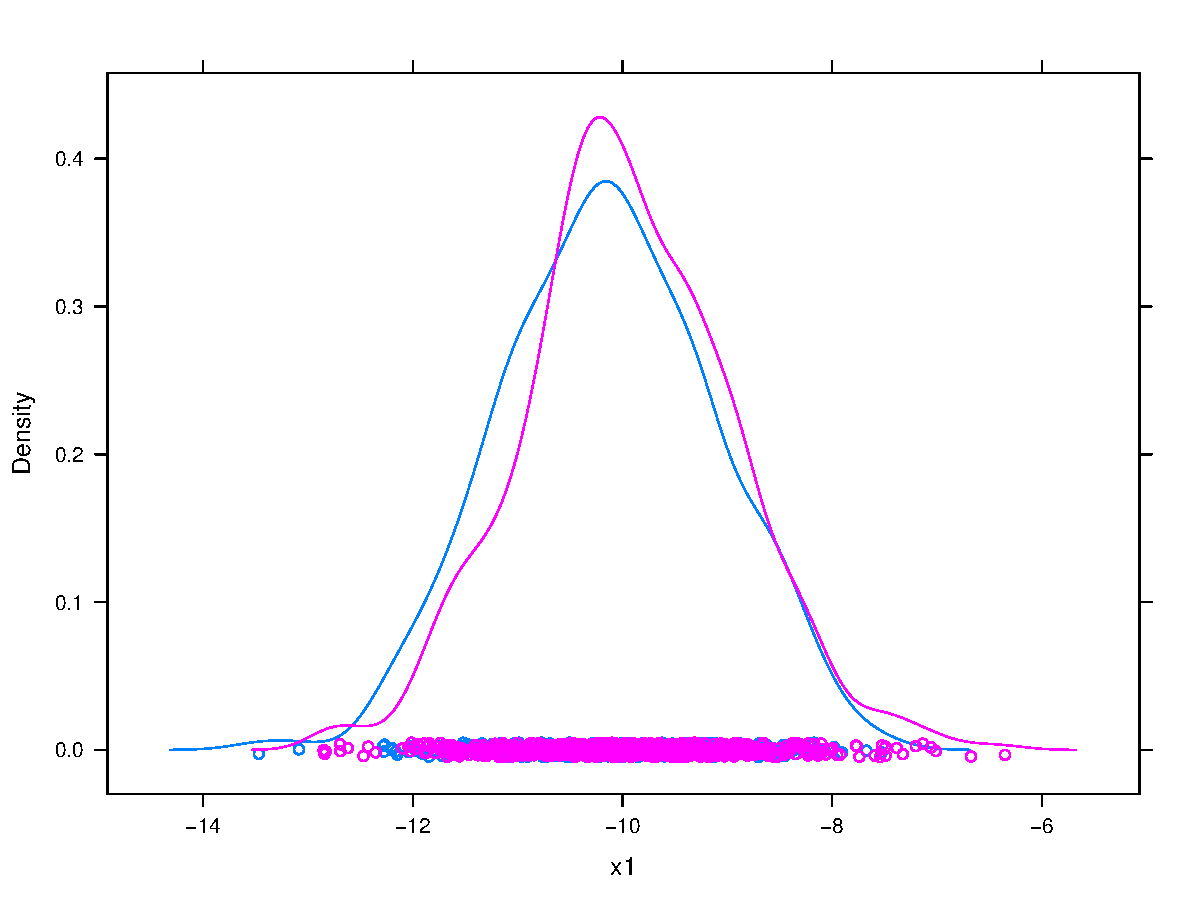
\includegraphics[width=\maxwidth]{figure/sim:3-1} 

}


\begin{kframe}\begin{alltt}
\hlkwd{densityplot}\hlstd{(x2,} \hlkwc{groups} \hlstd{= z,} \hlkwc{data} \hlstd{= dat)}
\end{alltt}
\end{kframe}

{\centering 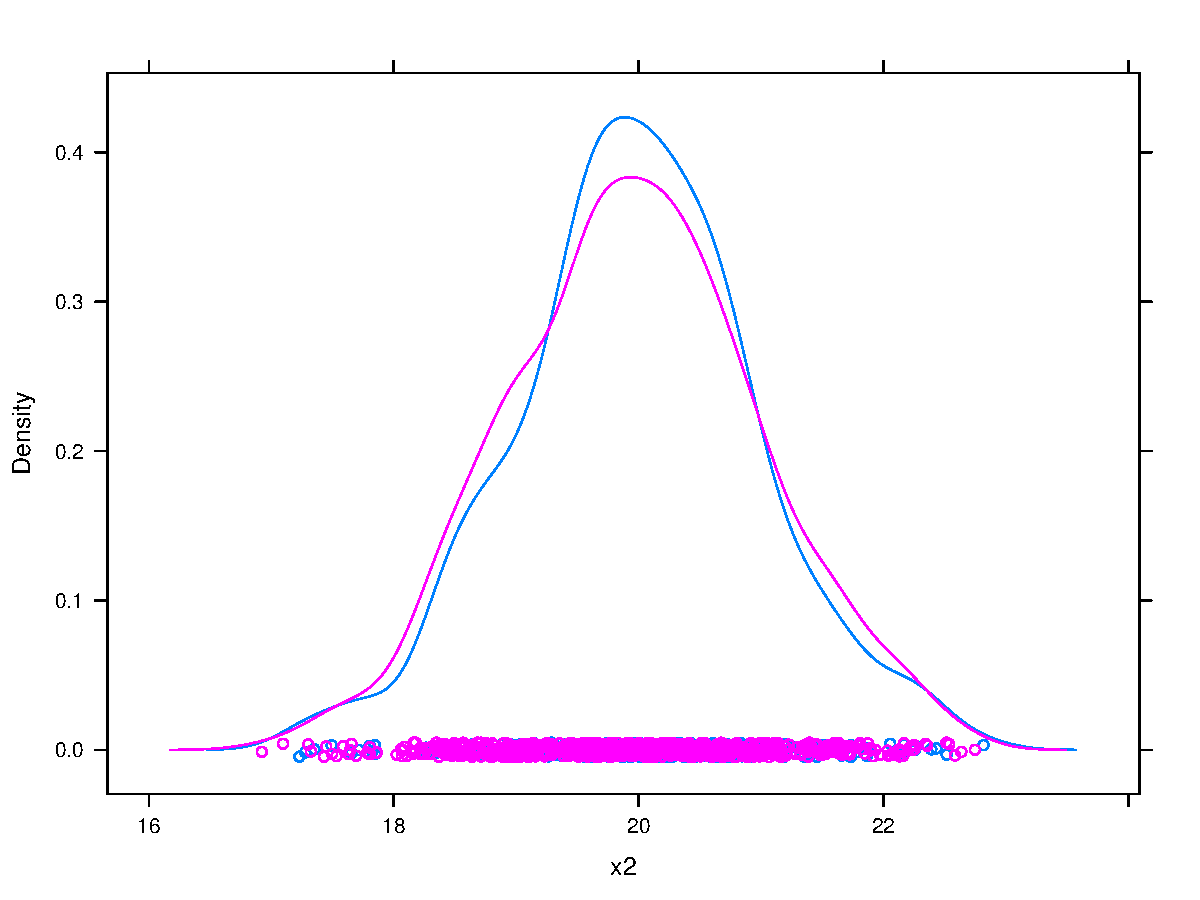
\includegraphics[width=\maxwidth]{figure/sim:3-2} 

}



\end{knitrout}

Hagamos matching.

\begin{knitrout}
\definecolor{shadecolor}{rgb}{0.969, 0.969, 0.969}\color{fgcolor}\begin{kframe}
\begin{alltt}
\hlcom{# install.packages("MatchIt", dependencies = T)}
\hlkwd{library}\hlstd{(}\hlstr{"MatchIt"}\hlstd{)}
\hlstd{m.out} \hlkwb{=} \hlkwd{matchit}\hlstd{(z} \hlopt{~} \hlstd{x1} \hlopt{+} \hlstd{x2,}
\hlkwc{data} \hlstd{= dat,}
\hlkwc{method} \hlstd{=} \hlstr{"nearest"}\hlstd{,} \hlcom{# nearest: "nearest neighbor"}
\hlkwc{discard} \hlstd{=} \hlstr{"both"}\hlstd{,}  \hlcom{# botar obs en ambas (T y C)}
\hlkwc{distance} \hlstd{=} \hlstr{"logit"}\hlstd{,}
\hlkwc{caliper} \hlstd{=} \hlnum{.1} \hlcom{# ventana de comparacion entre T y C}
\hlstd{)}
\end{alltt}
\end{kframe}
\end{knitrout}

Veamos si hubo mejoras.

\begin{knitrout}
\definecolor{shadecolor}{rgb}{0.969, 0.969, 0.969}\color{fgcolor}\begin{kframe}
\begin{alltt}
\hlkwd{summary}\hlstd{(m.out)} \hlcom{# inspeccionar balance y obs botadas}
\end{alltt}
\begin{verbatim}
## 
## Call:
## matchit(formula = z ~ x1 + x2, data = dat, method = "nearest", 
##     distance = "logit", discard = "both", caliper = 0.1)
## 
## Summary of Balance for All Data:
##          Means Treated Means Control Std. Mean Diff. Var. Ratio eCDF Mean
## distance        0.6807        0.6729          0.1891     0.9796    0.0508
## x1             -9.9522      -10.1411          0.1872     1.0032    0.0498
## x2             19.9585       19.9825         -0.0233     1.1028    0.0160
##          eCDF Max
## distance   0.1001
## x1         0.0967
## x2         0.0514
## 
## 
## Summary of Balance for Matched Data:
##          Means Treated Means Control Std. Mean Diff. Var. Ratio eCDF Mean
## distance        0.6781        0.6746          0.0845     1.0078    0.0261
## x1            -10.0172      -10.1043          0.0864     1.0074    0.0255
## x2             19.9823       19.9693          0.0125     1.1600    0.0170
##          eCDF Max Std. Pair Dist.
## distance   0.0520          0.0848
## x1         0.0694          0.1553
## x2         0.0405          1.1098
## 
## Percent Balance Improvement:
##          Std. Mean Diff. Var. Ratio eCDF Mean eCDF Max
## distance            55.3       62.2      48.6     48.1
## x1                  53.9     -130.4      48.7     28.3
## x2                  46.1      -51.6      -6.8     21.3
## 
## Sample Sizes:
##           Control Treated
## All           354     746
## Matched       346     346
## Unmatched       7     387
## Discarded       1      13
\end{verbatim}
\end{kframe}
\end{knitrout}

Sigamos inspeccionando de manera visual.

\begin{knitrout}
\definecolor{shadecolor}{rgb}{0.969, 0.969, 0.969}\color{fgcolor}\begin{kframe}
\begin{alltt}
\hlkwd{plot}\hlstd{(m.out,} \hlkwc{type} \hlstd{=} \hlstr{"jitter"}\hlstd{,} \hlkwc{interactive} \hlstd{=} \hlnum{FALSE}\hlstd{,} \hlkwc{col} \hlstd{=} \hlstr{"blue"}\hlstd{)}
\end{alltt}
\end{kframe}

{\centering 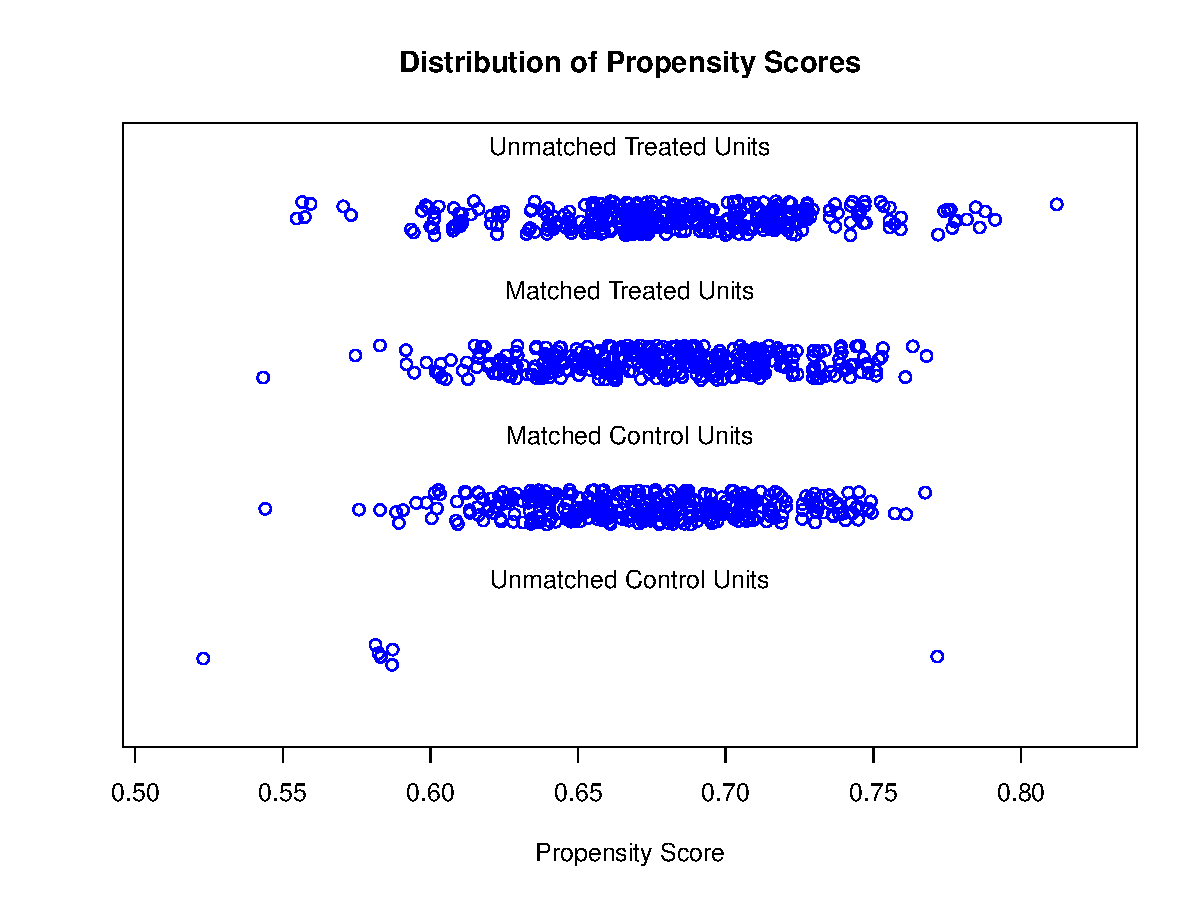
\includegraphics[width=\maxwidth]{figure/sim:6-1} 

}


\begin{kframe}\begin{alltt}
\hlkwd{plot}\hlstd{(m.out,} \hlkwc{type} \hlstd{=} \hlstr{"hist"}\hlstd{)}
\end{alltt}
\end{kframe}

{\centering 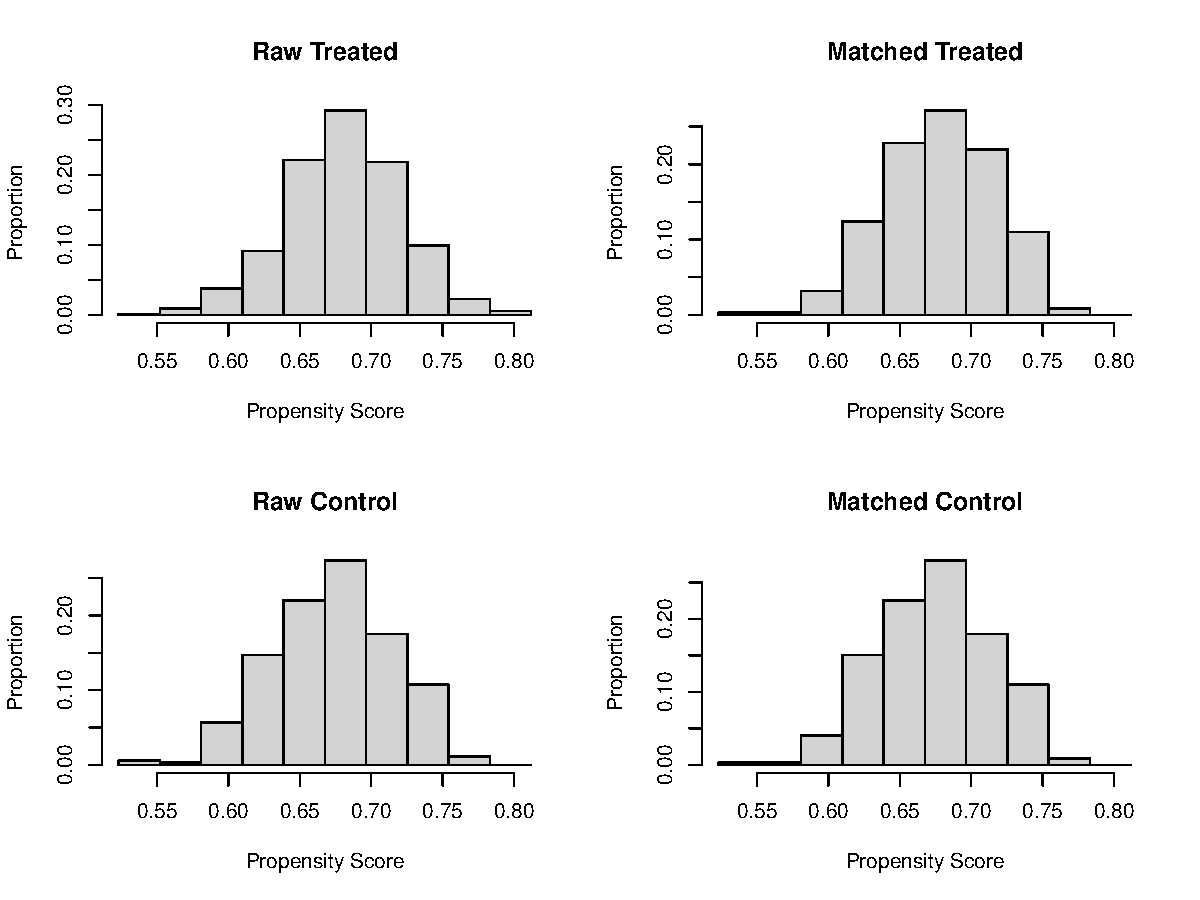
\includegraphics[width=\maxwidth]{figure/sim:6-2} 

}


\begin{kframe}\begin{alltt}
\hlkwd{plot}\hlstd{(m.out,} \hlkwc{type} \hlstd{=} \hlstr{"qq"}\hlstd{,} \hlkwc{interactive} \hlstd{=} \hlnum{FALSE}\hlstd{)}
\end{alltt}
\end{kframe}

{\centering 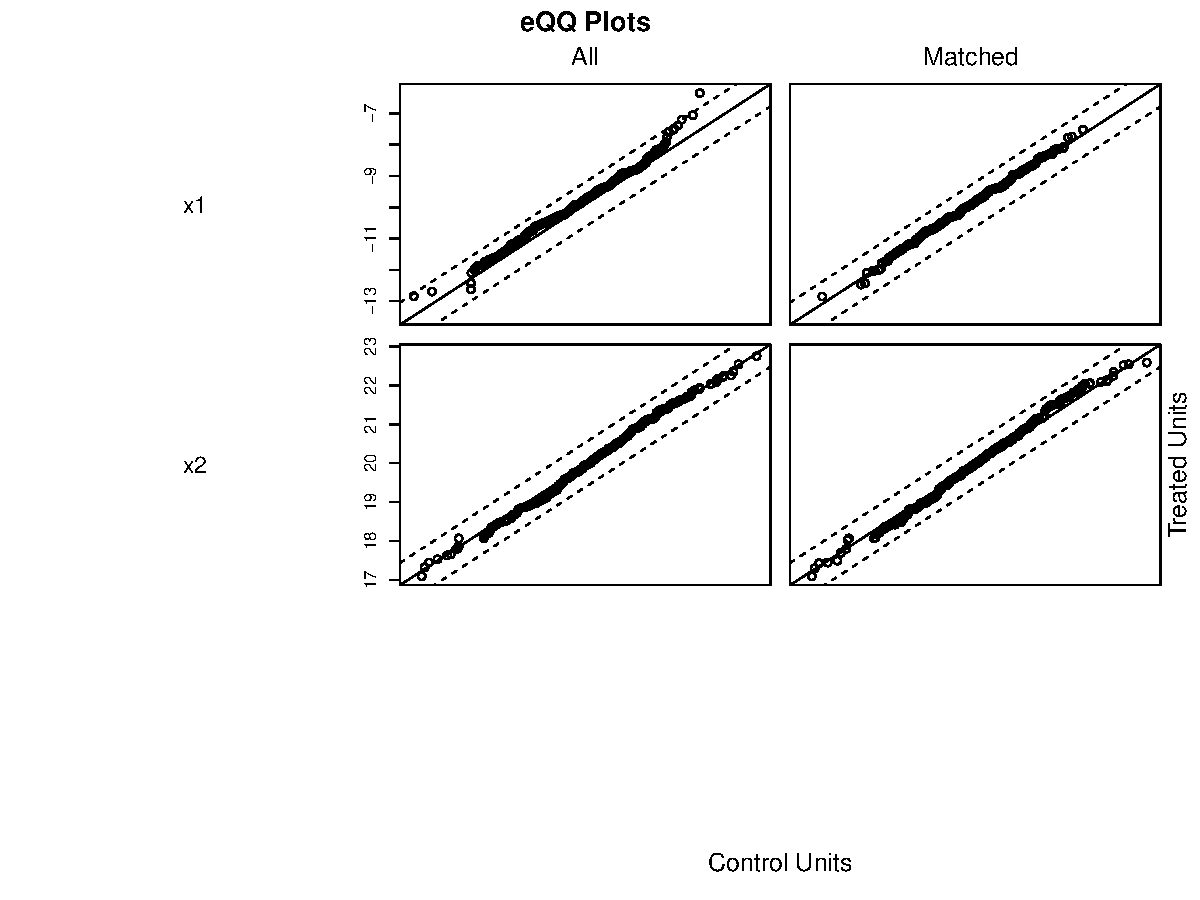
\includegraphics[width=\maxwidth]{figure/sim:6-3} 

}



\end{knitrout}

OK. Ahora, botemos las observaciones creando una base de datos nueva \texttt{m.data}.

\begin{knitrout}
\definecolor{shadecolor}{rgb}{0.969, 0.969, 0.969}\color{fgcolor}\begin{kframe}
\begin{alltt}
\hlstd{m.data} \hlkwb{=} \hlkwd{match.data}\hlstd{(m.out,} \hlkwc{distance} \hlstd{=} \hlstr{"prop.score"}\hlstd{,} \hlkwc{drop.unmatched} \hlstd{= T)} \hlcom{# construir DF}
\end{alltt}
\end{kframe}
\end{knitrout}

Ahora, estimemos dos modelos, uno con todos los datos (``\emph{raw}'') y otro con los datos \emph{matcheados} (``\emph{matched}'').

\begin{kframe}
\begin{alltt}
\hlstd{raw.m} \hlkwb{=} \hlkwd{lm}\hlstd{(y} \hlopt{~} \hlstd{z} \hlopt{+} \hlstd{x1} \hlopt{+} \hlstd{x2,} \hlkwc{data} \hlstd{= dat)} \hlcom{# OLS (Raw)}
\hlstd{matched.m} \hlkwb{=} \hlkwd{lm}\hlstd{(y} \hlopt{~} \hlstd{z} \hlopt{+} \hlstd{x1} \hlopt{+} \hlstd{x2,} \hlkwc{data} \hlstd{= m.data)} \hlcom{# OLS (Matched)}
\hlkwd{library}\hlstd{(texreg)}
\hlkwd{texreg}\hlstd{(}\hlkwd{list}\hlstd{(raw.m, matched.m))}
\end{alltt}
\end{kframe}
\begin{table}
\begin{center}
\begin{tabular}{l c c}
\hline
 & Model 1 & Model 2 \\
\hline
(Intercept) & $-0.56$      & $-1.05$      \\
            & $(0.68)$     & $(0.91)$     \\
z           & $1.06^{***}$ & $0.98^{***}$ \\
            & $(0.07)$     & $(0.08)$     \\
x1          & $0.99^{***}$ & $0.96^{***}$ \\
            & $(0.03)$     & $(0.04)$     \\
x2          & $2.02^{***}$ & $2.03^{***}$ \\
            & $(0.03)$     & $(0.04)$     \\
\hline
R$^2$       & $0.84$       & $0.84$       \\
Adj. R$^2$  & $0.84$       & $0.84$       \\
Num. obs.   & $1100$       & $692$        \\
\hline
\multicolumn{3}{l}{\scriptsize{$^{***}p<0.001$; $^{**}p<0.01$; $^{*}p<0.05$}}
\end{tabular}
\caption{Statistical models}
\label{table:coefficients}
\end{center}
\end{table}





\begin{knitrout}
\definecolor{shadecolor}{rgb}{0.969, 0.969, 0.969}\color{fgcolor}\begin{kframe}
\begin{alltt}
\hlstd{knitr}\hlopt{::}\hlkwd{purl}\hlstd{(}\hlstr{'Matching.Rnw'}\hlstd{)}
\end{alltt}


{\ttfamily\noindent\bfseries\color{errorcolor}{\#\# Error in parse\_block(g[-1], g[1], params.src, markdown\_mode): Duplicate chunk label 'setup', which has been used for the chunk:\\\#\# if (!require("{}pacman"{})) install.packages("{}pacman"{}); library(pacman)\\\#\# p\_load(knitr)\\\#\# set.seed(2020)\\\#\# options(scipen=9999999)}}\begin{alltt}
\hlkwd{Stangle}\hlstd{(}\hlstr{'Matching.Rnw'}\hlstd{)}
\end{alltt}
\begin{verbatim}
## Writing to file Matching.R
\end{verbatim}


{\ttfamily\noindent\bfseries\color{errorcolor}{\#\# Error in match.arg(options\$results, c("{}verbatim"{}, "{}tex"{}, "{}hide"{})): 'arg' should be one of "{}verbatim"{}, "{}tex"{}, "{}hide"{}}}\end{kframe}
\end{knitrout}


\newpage
\paragraph{}
\paragraph{}
\pagenumbering{Roman}
\setcounter{page}{1}
\printbibliography



\end{document}

